\section{Implementation, CPU/GPU Comparison, and Resources}
\label{chapter:10}

% block-id: 10.compute.heading
\hypertarget{10.compute.heading}{}
\subsection{CPU/GPU numerical comparison and computational scale}

% block-id: 10.compute.p1
\hypertarget{10.compute.p1}{}
With identical model, discretization, and integration settings, the 5024-degree-of-freedom CPU/GPU partial-inductance matrices differ relatively by 7.48×10⁻¹⁶ and their complex currents by 7.78×10⁻¹⁴. The 1264-degree-of-freedom case also meets the 10⁻¹⁰ comparison threshold, as shown in Fig.~\ref{fig:gpu_equivalence}. These results establish numerical agreement between the two implemented algorithms for the compared matrices and port solutions. Performance comparisons additionally require matching timing boundaries; stage times and resource samples are retained, while physical conclusions rely on the model checks described above.

% block-id: 10.compute.p2
\hypertarget{10.compute.p2}{}
Fig.~\ref{fig:resource_memory} shows sampled memory usage for identifiable owned process trees; short peaks between samples may exceed the displayed curve. At larger scales, the 9856-degree-of-freedom case retains recoverable partial currents and related results, while its complete matrix, common voltage and full-field coverage are itemized in the data inventory. Cases with 20108 or more degrees of freedom record resource requirements and termination boundaries. These records inform the cost of further computation; complete numerical verification rests on cases with the corresponding acceptance data.

% block-id: 10.workflow.heading
\hypertarget{10.workflow.heading}{}
\subsection{Computation and document construction}

% block-id: 10.workflow.p1
\hypertarget{10.workflow.p1}{}
Research entry points read model inputs and solver settings and produce run records and corresponding checks. Publication entry points read saved quantities, figures and canonical LaTeX prose to generate Markdown reading editions and compile preview PDFs. Input, source, and output hashes identify each build. Individual figures retain vector curves and font information, while composites record panel identities and layout parameters. The following source table links observables in the text to specific files and acceptance records.

% block-id: 10.figure.gpu_equivalence
\hypertarget{10.figure.gpu_equivalence}{}
\begin{figure}[!htbp]
\centering
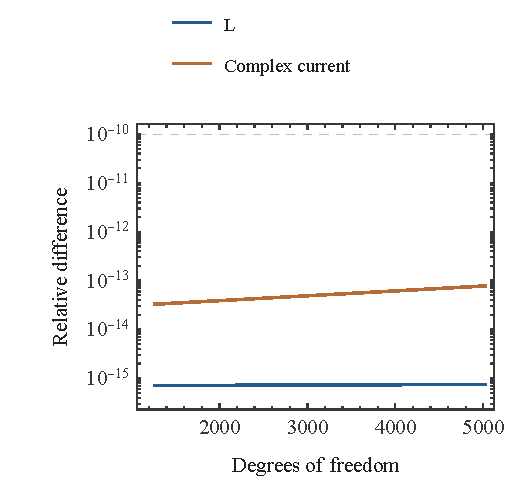
\includegraphics[width=\linewidth,height=.72\textheight,keepaspectratio]{../../assets/en/gpu_equivalence.pdf}
\caption{CPU/GPU same-model numerical comparison. Relative matrix and complex-current differences use identical discretization and integration. Relative differences are computed separately for 1264 and 5024 degrees of freedom. The horizontal reference is the 10⁻¹⁰ algorithm-comparison target.}
\label{fig:gpu_equivalence}
\end{figure}

% block-id: 10.figure.resource_memory
\hypertarget{10.figure.resource_memory}{}
\begin{figure}[!htbp]
\centering
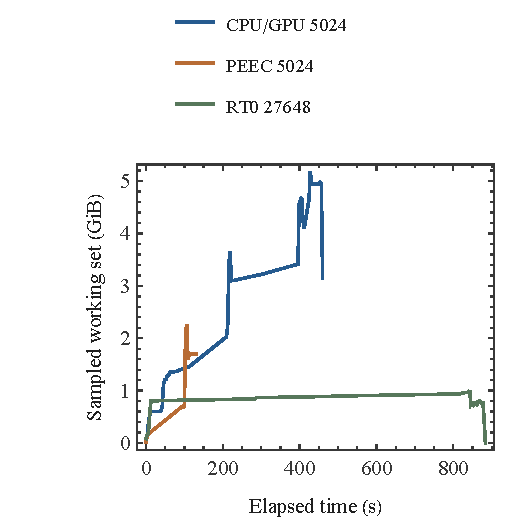
\includegraphics[width=\linewidth,height=.72\textheight,keepaspectratio]{../../assets/en/resource_memory.pdf}
\caption{Attributable process-tree resource curves. Curves use archived time and memory samples. Time is measured from the start of each corresponding run. Memory is the sampled working set of the attributable process tree.}
\label{fig:resource_memory}
\end{figure}
